% Created 2024-09-23 Mon 13:35
% Intended LaTeX compiler: pdflatex
%%% TeX-command-extra-options: "-shell-escape"

\documentclass{iacrtrans}
\usepackage[utf8]{inputenc}
\usepackage[T1]{fontenc}

% -- Default Packages --
\usepackage{graphicx}
\usepackage{longtable}
\usepackage{wrapfig}
\usepackage{rotating}
\usepackage{tcolorbox}
\tcbuselibrary{skins}
\usepackage{booktabs}
% \usepackage{multirow}
\usepackage[normalem]{ulem}
\usepackage{amsmath}
\usepackage{amssymb}
\usepackage{capt-of}
\usepackage{hyperref}
\usepackage{tikz}

\newtcolorbox{empheqboxed}{
  enhanced,
  boxsep=1pt,
  arc=0.75ex,
  colback=gray!10,
  colframe=gray!40,
  boxrule=1pt,
  leftrule=40pt,
  top=-3.5mm,
  overlay unbroken and first ={%
    \node[minimum width=1cm,
      anchor=south,
      font=\sffamily\bfseries,
      xshift=20pt,
      yshift=-6.5pt,
    black]
    at (frame.west) {Stack:};
  }
}

\newcommand{\mycomment}[1]{}
\newcommand{\elem}[1]{\, \langle #1 \rangle \,}
\newcommand{\opcode}[1]{\, \texttt{#1} \,}
\newcommand{\script}[1]{ $\big\{ #1 \big\}$ }

\makeatletter
\newcommand{\citeprocitem}[2]{\hyper@linkstart{cite}{citeproc_bib_item_#1}#2\hyper@linkend}
\makeatother

\author{Kyrylo Baibula \inst{1} \and Oleksandr Kurbatov\inst{1} \and
Dmytro Zakharov\inst{1}}
\institute{Distributed Lab
  \email{dmytro.zakharov@distributedlab.com},
\email{ok@distributedlab.com}, \email{kyrylo.baybula@distributedlab.com}}
\title[Verifiable Computation on Bitcoin]{Generic Optimistic
Verifiable Computation on Bitcoin: BitVM2 Approach}

\hypersetup{
  pdfauthor={Distributed Lab},
  pdftitle={BitVM Fast Recap},
  pdfkeywords={},
  pdfsubject={},
  pdfcreator={Emacs 29.4 (Org mode 9.7.11)},
pdflang={English}}

\usepackage{biblatex}
\addbibresource{refs.bib}

\begin{document}

\maketitle

\keywords[]{Bitcoin, Bitcoin Script, Verifiable Computation,
Optimistic Verification, BitVM2}

\begin{abstract}
  Assume some user wants to publicly execute a large program on the
  Bitcoin chain, but its implementation in the native for Bitcoin
  scripting language --- Bitcoin Script --- is larger than 4 megabytes
  (for example, a zero-knowledge verification logic), making it
  impossible to publish the complex logic on-chain input. This
  document is a fast recap of the BitVM2 doc, which proposes
  optimistic execution verification with fraud proofs in case of
  incorrectness.
\end{abstract}

\setcounter{tocdepth}{2}
\tableofcontents

\section{Introduction}\label{sec:intro}

In the ever-evolving landscape of blockchain technology, the desire to
execute increasingly complex and large-scale programs on the
Bitcoin\autocite{bitcoin_paper} network is growing. However, Bitcoin
Script, the native programming language of Bitcoin, imposes strict
size limits, such as the 4-megabyte cap on transaction inputs, which
makes it challenging to implement certain advanced cryptographic
proofs, like zero-knowledge proofs verification on-chain. To address
this limitation, the BitVM2\autocite{bitvm2} proposal introduces an
innovative approach that enables the optimistic execution of large
programs on the Bitcoin chain. This method leverages fraud proofs to
ensure the validity of executions, offering a robust mechanism for
verifying computations, while providing a fail-safe against incorrect
or malicious operations. This document provides a concise overview of
BitVM2, highlighting its potential to unlock new possibilities for
secure and scalable program execution on Bitcoin.

\section{Program splitting}\label{sec:program-splitting}

\begin{quote}
  Let there be a large program \(f\), which can be described in
  Bitcoin Script. We want to compute it \textbf{on-chain}, i.e., find
  such an \(f(x) = y\). To achieve this, we divide the program into
  \(n\) sub-programs \(f_1, \ldots, f_n\) and their corresponding
  intermediate states \(z_1, \ldots, z_n\), such that:

  \begin{equation}
    \begin{aligned}
      f_1(x) &= z_1 \\
      f_2(z_1) &= z_2 \\
      &\cdots \\
      f_n(z_{n-1}) &= y
    \end{aligned}
  \end{equation}
\end{quote}

However, the user (referred in BitVM2 as the operator) only needs to
prove that the given program \(f\) indeed returns \(y\) for \(x\), or
\textbf{give others the opportunity to disprove this fact}. In our
case, this means giving challengers the ability to prove that for at
least one of the sub-programs statement \(f_i(z_{i-1}) \neq z_i\) is
true.

\section{\textbf{Assert} transaction}\label{sec:assert-tx}

To achieve this, the user publishes an \textbf{Assert} transaction,
which has one output with multiple possible spending scenarios:

\begin{enumerate}
  \item \textbf{PayoutScript} (\textbf{LockTime} + signature) --- the
    transaction has passed verification, and the operator can spend the
    output, thereby confirming the statement \(f(x) = y\).
  \item \textbf{DisproveScript} --- one of the challengers has found a
    discrepancy in the intermediate states \(z_i\), \(z_{i-1}\) and the
    sub-program \(f_i\). In other words, they have proven that
    \(f_i(z_{i-1}) \neq z_i\), and thus, they can spend the output.
    p
\end{enumerate}

\subsection{\texttt{DispoveScript}}\label{sec:dispove-script}

\texttt{DispoveScript} is part of the MAST tree in a Taproot address,
which allows challengers to claim the transaction amount for states
\(z_i\), \(z_{i-1}\), and sub-program \(f_i\), is called
\(\mathsf{DisproveScript}_i\) in BitVM2:

\begin{verbatim}
// push z_i, z_{i-1} onto the stack
{ z_i     }
{ z_(i-1) }
// compute f(z_{i-1})
{ f_i     }
// ensure that f_i(z_{i-1}) != z_i
OP_EQUAL
OP_NOT
\end{verbatim}

In fact, this script does not need a \texttt{script\_sig}, as with the
correct \(z_i\) and \(z_{i-1}\), it will always execute
successfully. Therefore, to restrict spending capability, a Winternitz
signature and Covenants verification are added to the script.

\subsubsection{Winternitz Signature}\label{sec:lamport-signature}

Unlike other digital signature algorithms, the Winternitz signature
uses a pair of random secret and public keys
$(\mathsf{sk}, \mathsf{pk})$ that can sign and verify only any message
from the message space \(\mathcal{M} = {\{0, 1\}}^{\ell}\) of
$\ell$-bit messages.

However, once the signature $\sigma_{m}$ is formed, where
$m \in \mathcal{M}$ is the message being signed,
\((\mathsf{sk}_{m}, \mathsf{pk}_{m})\) become tied to \(m\), because
any other signature with these keys will compromise the keys
themselves. Thus, for the message \(m\), the keys
\((\mathsf{sk}_{m}, \mathsf{pk}_{m})\) are one-time use.

Now, let us define the Winternitz Signature. Further by $f^{(k)}(x)$
denote the composition of function $f$ with itself $k$ times:
$f^{(k)}(x) = \underbrace{f \circ \dots \circ f}_{k \; \text{times}}(x)$.

\begin{definition}
  The \textbf{Winternitz Signature Scheme} over parameters $(k,d)$
  with a hash function $H: \mathcal{X} \to \mathcal{X}$ is defined as follows:
  \begin{itemize}
    \item $\mathsf{Gen}(1^{\lambda})$: secret key is generated as a tuple
      $(x_1,\dots,x_k) \xleftarrow{R} \mathcal{X}$, while the public key is
      $(y_1,\dots,y_k)$, where $y_j = H^{(d)}(x_j)$ for each
      $j \in \{1,\dots,k\}$.
    \item $\mathsf{Sign}(m,\mathsf{sk})$: denote by
      $\mathcal{I}_{d,k} := {(\{0,\dots,d\})}^k$ and suppose we have an encoding
      function $\mathsf{Enc}: \mathcal{M} \to \mathcal{I}_{d,k}$ that
      translates a message
      $m \in \mathcal{M} = {\{0,1\}}^{\ell}$ to the element in space
      $\mathcal{I}_{d,k}$. Now, set
      $e = (e_1,\dots,e_k) \gets \mathsf{Enc}(m)$. Then, the signature is
      formed as:
      \begin{equation*}
        \sigma \gets ({H}^{(e_1)}(x_1), H^{(e_2)}(x_2), \dots, H^{(e_k)}(x_k))
      \end{equation*}
    \item $\mathsf{Verify}(\sigma,m,\mathsf{pk})$: to verify
      $\sigma = (\sigma_1,\dots,\sigma_k)$ on $m \in \mathcal{M}$ and
      $\mathsf{pk}=(y_1,\dots,y_k)$, first compute encoding
      $(e_1,\dots,e_k) \gets \mathsf{Enc}(m)$ and then check whether:
      \begin{equation*}
        H^{(d-e_j)}(\sigma_j) = y_j, \quad j \in \{1,\dots,k\}.
      \end{equation*}
  \end{itemize}
\end{definition}

That being said, by taking the intermediate states
${\{z_j\}}_{1 \leq j \leq n}$ as the message for the Winternitz signature, we
form one-time key pairs
${\{(\mathsf{sk}_j,\mathsf{pk}_j)\}}_{1 \leq j \leq n}$ and signatures
${\{\sigma_j\}}_{1 \leq j \leq n}$, respectively (where each of
  $\mathsf{pk}_j$, $\mathsf{sk}_j$, and $\sigma_j$ corresponds to the
intermediate variable $z_j$). Then, to spend the output from the
\texttt{Assert} transaction using the $\texttt{DisproveScript}_j$
script, the challenger is required to add the corresponding states
$z_j$, $z_{j-1}$, and corresponding signatures $\sigma_j$,
$\sigma_{j-1}$ to the stack in the \texttt{scriptSig}, making the
\texttt{scriptSig} of the transaction input like this:

\begin{empheqboxed}
  \begin{align*}
    &\elem{z_{j-1}} \opcode{OP\_DUP} \elem{\sigma_{j-1}}
    \elem{\mathsf{pk}_{j-1}} \opcode{OP\_WINTERNITZVERIFY} \\
    &\elem{z_{j}} \opcode{OP\_DUP} \elem{\sigma_{j}}
    \elem{\mathsf{pk}_{j}} \opcode{OP\_WINTERNITZVERIFY} \\
    &\elem{f_j} \opcode{OP\_EQUAL} \opcode{OP\_NOT}
  \end{align*}
\end{empheqboxed}

where \texttt{OP\_WINTERNITZVERIFY} is the verification of the
Winternitz signature (commitment), described in Bitcoin Script (as
  Bitcoin Script does not have a built-in \texttt{OP\_CODE} for
Winternitz signatures)\footnote{Its implementation can be found here:
\url{https://github.com/distributed-lab/bitvm2-splitter/blob/feature/winternitz/bitcoin-winternitz/src/lib.rs}.}.

The correct implementation of \texttt{OP\_WINTERNITZVERIFY} in Bitcoin
Script would require the $\mathsf{Enc}(m)$ to split the state into $d$
digit numbers or recover the state from $d$ digit numbers on stack,
which without the bitwise operations or \texttt{OP\_CAT} for larger
than 32-bit values is nearly impossible.

\subsubsection{Winternitz Signatures in Bitcoin
  Script}\label{sec:winternitz-in-bitcoin-script}

Instead of bitwise operations, the Bitcoin script can use arithmetic
ones. Still, this arithmetic is limited and contains only basic
opcodes such as \texttt{OP\_ADD}. To make matters worse, all the
corresponding operations can be applied to 32-bit elements only, and
as the last one is reserved for a sign, only 31 bits can be used to
store the state. This limitation can be considered strong, but most of
the math can be implemented through 32-bit stack elements. So lets fix
$\ell = 32$ --- maximum size of the stack element in bits.

By defining the $\mathsf{Enc}(m)$ as a domination free function
$P(m)$, like described in~\cite{applied-crypto}, it is convenient to
make $d+1$ the power of two. Therefore, from now on, we set
$d+1 = 2^w$ for some $w \in \mathbb{N}$. Which splits $m$ by some number of equal
chunks of $w$ bits, and $k$ becomes the sum of $n_0$ --- the number of
$d$-digit numbers from $m$, and $n_1$ a checksum (see
table~\ref{tab:winternitz}).

\iffalse{}
%The python script i used for this table:
\begin{verbatim}
import math
l = 32
ds = [3, 7, 15, 31, 63, 127, 255]

for d in ds:
    w = math.ceil(math.log(d+1, 2))
    n0 = math.ceil(l / w)
    n1 = math.ceil((2**w * n0).bit_length() / w)
    k = n0 + n1
    print(f"{w} & {n0} & {n1} & {k} \\\\")
\end{verbatim}
\fi

\begin{table}[h]
  \centering
  \begin{tabular}{lcccc}
    \toprule
    $w$ & $n_0$ & $n_1$ & $k$ \\
    \midrule
    2 & 16 & 4 & 20 \\
    3 & 11 & 3 & 14 \\
    4 & 8 & 2 & 10 \\
    5 & 7 & 2 & 9 \\
    6 & 6 & 2 & 8 \\
    7 & 5 & 2 & 7 \\
    8 & 4 & 2 & 6 \\
    \bottomrule
  \end{tabular}
  \caption{Different values of $k$ depending on $d$ for 32-bit
  message}\label{tab:winternitz}
\end{table}

If chunks are of equal lengths, the recovery from $n_0$ digits is
simply:

\begin{equation}
  \begin{aligned}
    w &:= \log_2{(d+1)} \\
    m &= \sum_{i = 0}^{n_0} e_i \cdot 2^{i w}
  \end{aligned}
  \label{eq:u32-recovery}
\end{equation}

Where multiplication by powers of two can be implemented in Bitcoin
Script with sequence of \texttt{OP\_DUP} and \texttt{OP\_ADD}
opcodes. So, for example, multiplication of $e_j$ by $2^n$ in Bitcoin
Script is:

\begin{empheqboxed}
  \begin{align*}
    \elem{e_j} \underbrace{\opcode{OP\_DUP} \opcode{OP\_ADD}}_{n \; \text{times}}
  \end{align*}
\end{empheqboxed}

As Bitcoin Script has no loops or jumps, implementing dynamic number
of operations, like hashing something $d - e_j$ times without knowing
the $e_j$ before hand is challenging. That's why implementation uses
the ``lookup'' table of all $d$ hashes of signature's part $\sigma_j$ and
by using \texttt{OP\_PICK} pop the $d - e_j$ one on the top of stack,
like this:

\begin{empheqboxed}
  \begin{align*}
    & \elem{\sigma_j} \underbrace{\opcode{OP\_DUP}
    \opcode{OP\_HASH}}_{d \; \text{times}} \\
    & \elem{e_j} \opcode{OP\_PICK}
  \end{align*}
\end{empheqboxed}

Still the upper bound for script size in Bitcoin persists, but the
current implementation requires around 1000 bytes per 32-bit stack
element, which is unfortunatly a lot. Parts of the public key make the
largest contribution to the script size. Assuming that as $H$
implementation uses \texttt{OP\_HASH160}, each part $(y_1,\dots,y_k)$
of the public key $\mathsf{pk}_{m}$ adds 40 bytes to the total script
size. Additionaly, for calculating a lookup table for signature
verification, $2d \cdot k$ opcodes are used. Further more, for message
recovery $2 \sum_{i = 0}^{n_0} i w$ number of opcodes are added
too. Also, note that:

\begin{equation}
  \label{eq:opcodes-for-recovery-number}
    2 \sum_{i = 0}^{n_0} i w = w n_0 (n_0+1) \approx w n_0^2
\end{equation}

So the total script size, excluding utility opcodes, will be at least
$40k + 2 d k + w n_0 (n_0+1)$ (the sizes for different $d$ can be seen
in table~\ref{tab:winternitz-script-size}).

\iffalse{}
%The python script i used for this table:
\begin{verbatim}
import math
l = 32
ds = [3, 7, 15, 31, 63, 127, 255]

for d in ds:
    w = math.ceil(math.log(d+1, 2))
    n0 = math.ceil(l / w)
    n1 = math.ceil((2**w * n0).bit_length() / w)
    k = n0 + n1
    
    pk_size = 40 * k
    ver_size = 2 * d * k
    rec_size = 0
    for i in range(0, n0):
        rec_size += int(i * w)
    
    total = pk_size + ver_size + rec_size
    
    print(f"{d} & {pk_size} & {ver_size} & {rec_size} & {total} \\\\")
\end{verbatim}
\fi
\begin{table}[h]
  \centering
  \begin{tabular}{ccccc}
    \toprule
    $d$ & Public Key Size & Verification Script Size & Recovery
    Script Size & Total \\
    \midrule
    3 & 800 & 120 & 240 & 1160 \\
    7 & 560 & 196 & 165 & 921 \\
    15 & 400 & 300 & 112 & 812 \\
    31 & 360 & 558 & 105 & 1023 \\
    63 & 320 & 1008 & 90 & 1418 \\
    127 & 280 & 1778 & 70 & 2128 \\
    255 & 240 & 3060 & 48 & 3348 \\
    \bottomrule
  \end{tabular}
  \caption{Different script sizes depending on the $d$
  value per each 32-bit message}\label{tab:winternitz-script-size}
\end{table}

\subsection{Structure of the MAST Tree in a Taproot
Address}\label{sec:mast-tree-structure}

The inputs of the \texttt{Assert} transaction spend the output to a
Taproot address, which consists of a MAST tree of Bitcoin scripts
mentioned in Section~\ref{sec:assert-tx}. From the BitVM2 document, it
is known that the first \(n\) scripts in the tree are all
\(\mathsf{DisproveScript}_i\), where \(i = \overline{1, n}\), and the last is a
script that allows the operator who published the \texttt{Assert}
transaction to spend the output after some time. A visualization of
this tree can be seen in the figure~\ref{fig:assert-tx-mast-tree}.

\begin{figure}[htbp]
  \centering
  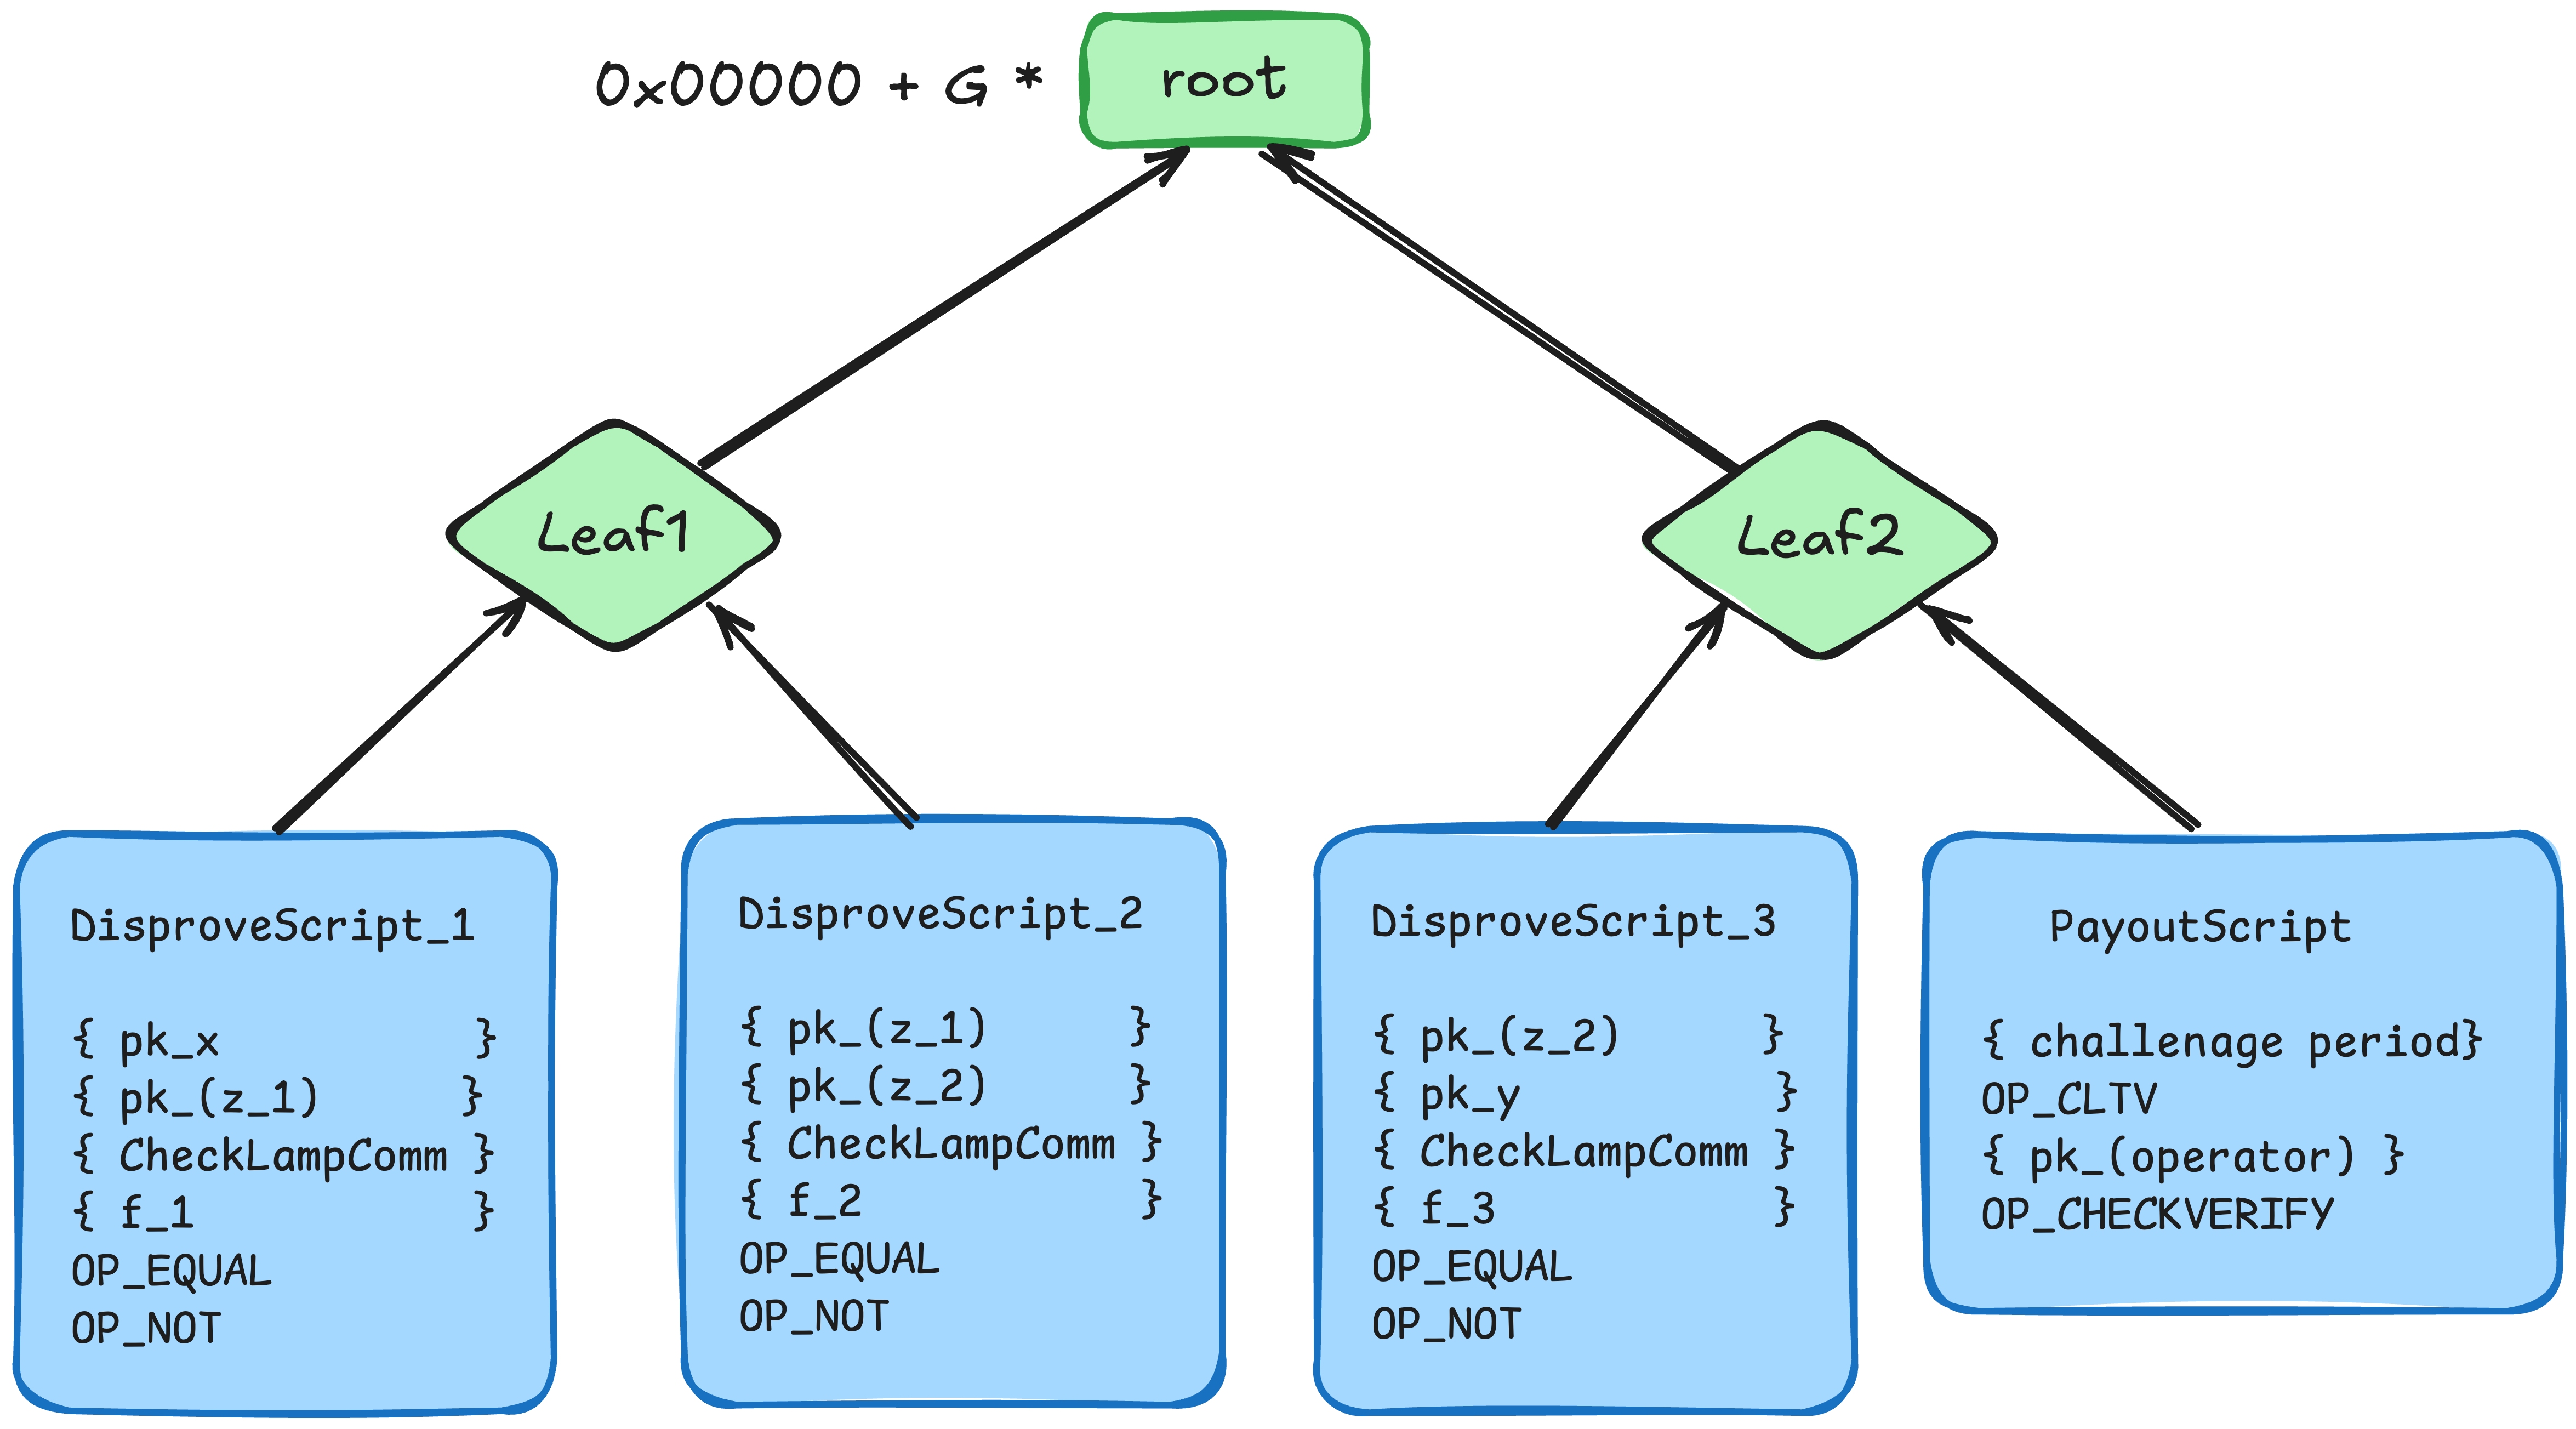
\includegraphics[width=.9\linewidth]{../images/assert-tx-taproot-output.png}
  \caption{\label{fig:assert-tx-mast-tree}Script tree in a Taproot
  address with three sub-programs and two intermediate states.}
\end{figure}

\section{\texttt{Disprove} and \texttt{Payout}
transactions}\label{sec:disprove-payout-txs}

These are transactions that spend the output from \texttt{Assert} via
\texttt{DisproveScript} and \texttt{PayoutScript} respectively (see
fig.~\ref{fig:bitvm-txs}). Their structure becomes more important when
we consider the emulation of ``covenants'' through a committee.

\begin{figure}[htbp]
  \centering
  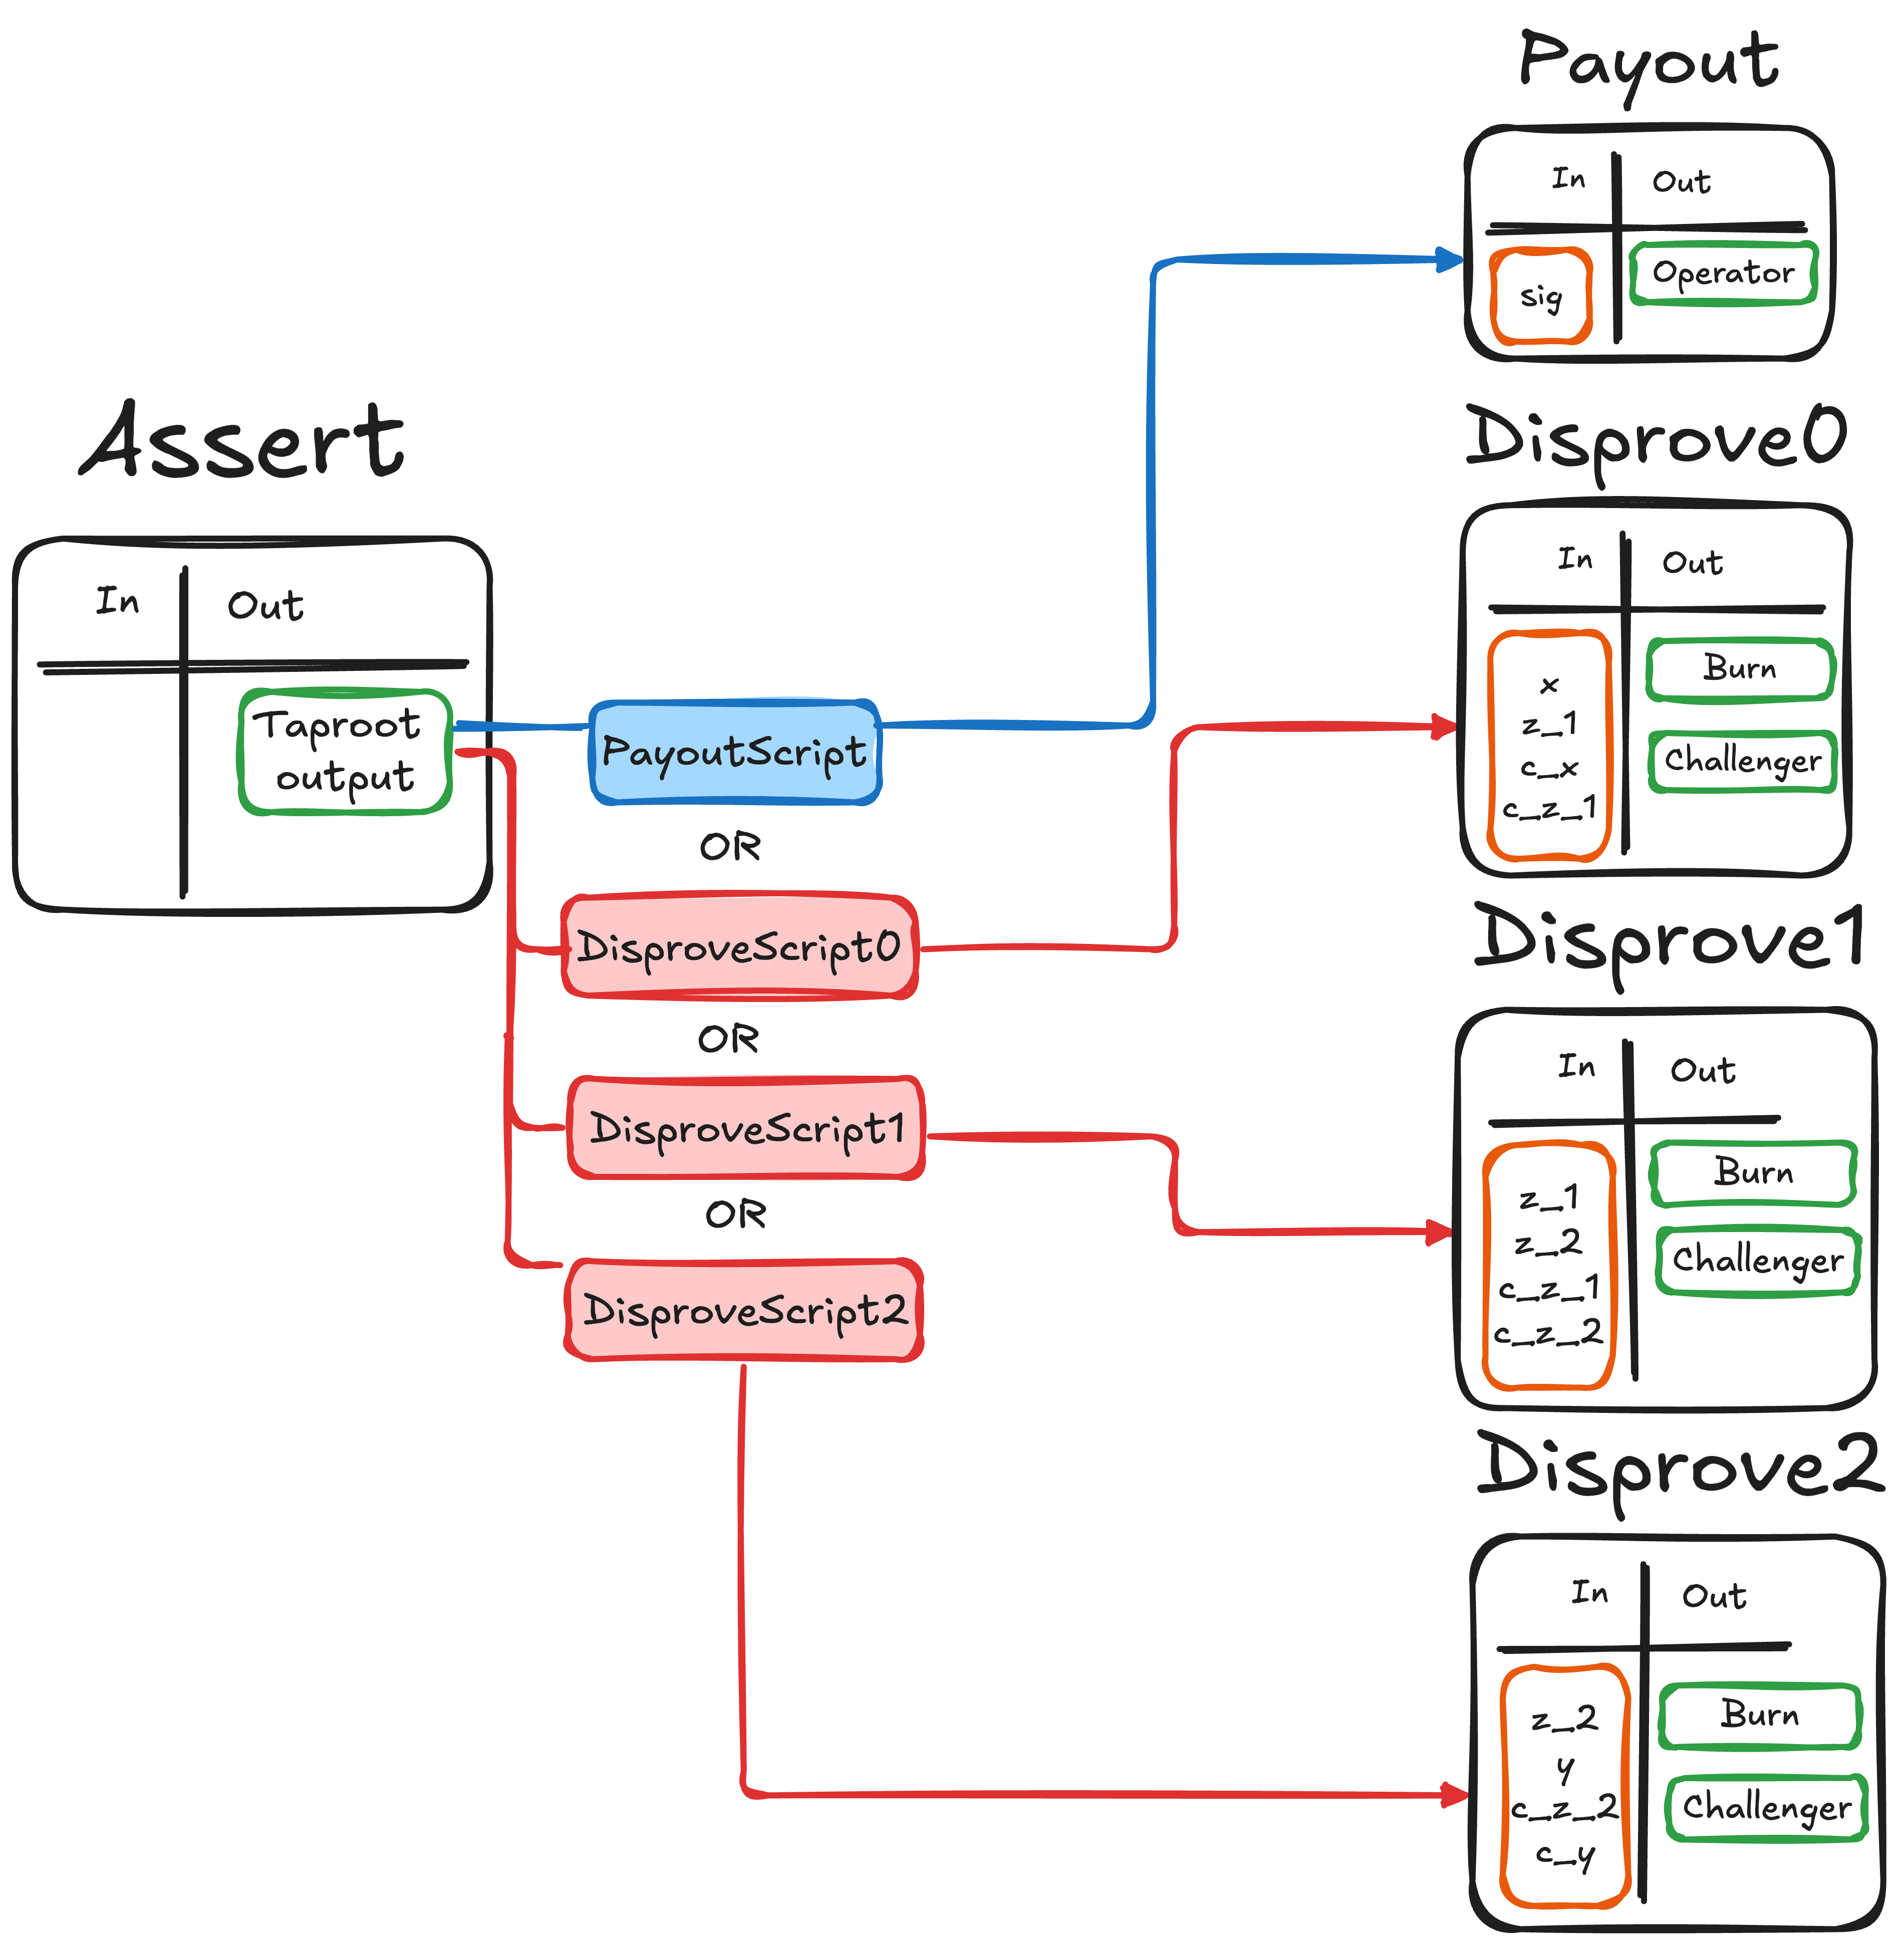
\includegraphics[width=.9\linewidth]{../images/bitvm-txs.png}
  \caption{\label{fig:bitvm-txs}Sequance of transactions in BitVM2
  with 3 subprograms and 2 intermediate states.}
\end{figure}

\section{{\bfseries\sffamily TODO} Covenants emulation through
comittee}\label{sec:covenants-emulation}

\printbibliography{}

\end{document}
